\newpage
\hypertarget{rules tex}{}
\subsection{Tex Rules}
\texHeader

Rules in the texual syntax are clearly separated into the three primary areas - the source, correspondence, and target - along with an area for constraints
which can manipulate attribute based on the transformation direction.

\subsection{BoxToDictionaryRule}

\begin{itemize}

\item[$\blacktriangleright$] You may have noticed that a \texttt{Rules} folder was created and included in the TGG package when you first created it. Create
your first TGG Rule by right-clicking on this folder and navigating to ``New/TGG Rule.'' Name it \texttt{BoxToDictionaryRule}, and confirm the file opens in the
editor window.

\item[$\blacktriangleright$] Lets first establish the \texttt{source} and \texttt{target}  structures. Given that this is the first rule to be applied in a
transformation, we can assume there is no context to work with, so each of our objects will need to be set to `green' (create). In the \texttt{source} scope,
create a \texttt{box} of type \texttt{Box}. Similarly, in the \texttt{target} scope, create a \texttt{dictionary} of type \texttt{Dictionary}. Your rule
should now resemble Fig.~\ref{eclipse:textSourceRule}.

\vspace{0.5cm}

\begin{figure}[htbp]
\begin{center}
  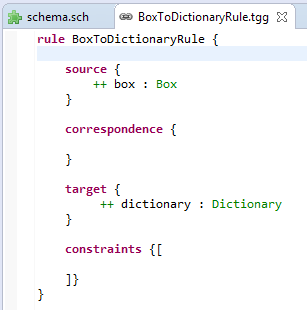
\includegraphics[width=0.5\textwidth]{eclipse_boxToDictionary_start}
  \caption{Setting the source and target objects}
  \label{eclipse:textSourceRule}
\end{center}
\end{figure}

\item[$\blacktriangleright$] Now we can create our first TGG Correspondence link! In the \texttt{correspondence} scope, enter 
\syntax{++ box <- boxToDictionary : BoxToDictionary -> dictionary}
Please note that the structure of this statement creates \emph{one} link, named \texttt{boxToDictionary}, of type \texttt{BoxToDictionary} which
was declared in the schema.

\end{itemize}

If this rule were to be run at this point, as-is, it would be actually successful by creating a single \texttt{Box} and \texttt{Dictionary}! Besides the
correspondence link however, these items have nothing in common. Let's try connecting the \texttt{name} of \texttt{box} to the \texttt{title} of \texttt{dictionary} with an
\emph{attribute constraint}. In TGG rules, attribute constraints provide a bidirectional and high level solution for attribute manipulations. In addition to the
basic math constraints such as addition (add), subtraction (sub), divide, max, multiply, and smallerOrEqual, we have some preexisting string constraints
we can use in this application. These include stringToNumber, concatenate (concant), addPrefix, addSuffix, and equals (eq).

\begin{itemize}

\item[$\blacktriangleright$] Therefore, under the \texttt{constraints} scope, write:
\syntax{eq(box.name, dictionary.title)}
Your rule should now resemble Fig.~\ref{eclipse:ruleBasic}.

\vspace{0.5cm}

\begin{figure}[htbp]
\begin{center}
  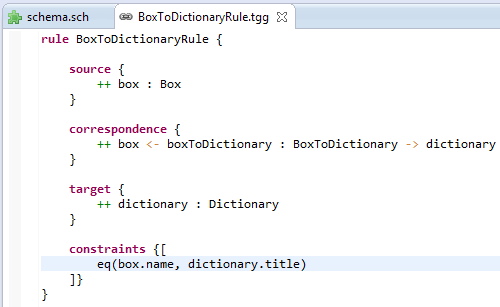
\includegraphics[width=0.8\textwidth]{eclipse_boxToDictionary_firstElements}
  \caption{Create a correspondence link and constraint}
  \label{eclipse:ruleBasic}
\end{center}
\end{figure}

\end{itemize}

Switch back to \texttt{BoxToDictionaryRule}. What's missing from our rule? We have created the primary container structures for the \texttt{target} and
\texttt{source}, but \texttt{cards} cannot be stored directly in \texttt{box}! We therefore need to create some \texttt{partition} objects. 

\begin{itemize}

\item[$\blacktriangleright$] Given that there are three difficulty \texttt{level}s for each dictionary \texttt{entry}, create three \texttt{partition}s to
store them in: \texttt{partition0}, \texttt{partition1}, and \texttt{partition2}. 

\vspace{0.5cm}

\item[$\blacktriangleright$] Complete the rule by setting both the individual \texttt{index} values and appropriate \texttt{containedPartition},
\texttt{next} and \texttt{previous} link variables so that your rule matches Fig.~\ref{eclipse:allReferences}.

\end{itemize}

\begin{figure}[htbp]
\begin{center}
  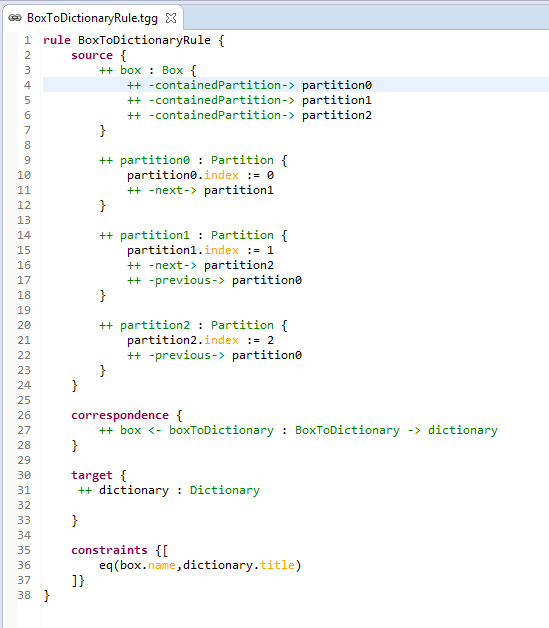
\includegraphics[width=0.8\textwidth]{eclipse_boxToDictionary_complete}
  \caption{\texttt{BoxToDictionaryRule} complete!}
  \label{eclipse:allReferences}
\end{center}
\end{figure}

\clearpage

Great work! This finished rule is able to transform a \texttt{box} into a \texttt{dictionary} and vice versa. Unfortunately, it will only be able to handle
completely empty boxes and dictionaries -- you can see we haven't provided any additional handling for \texttt{Card} or \texttt{Entry} items. If you're in a
hurry, feel free to jump ahead to Section 4: TGGs in Action, to try executing this rule anyway. Otherwise, the next rule we create will integrate itself with
\texttt{BoxToDictionaryRule} to take care of this.

% --------------- Card To Entry ------------------------------------------------------------------------------------------------------------------------
\subsection{CardToEntryRule}

\begin{itemize} 

\item[$\blacktriangleright$] Analogously to how you began the previous rule, return to the TGG schema and create a second correspondence type called
\texttt{CardToEntry}, with a \texttt{Card} source and \texttt{Entry} target. Your updated file should now resemble Fig.~\ref{eclipse:updatedSchema}.

\vspace{0.5cm}

\begin{figure}[htbp]
\begin{center}
  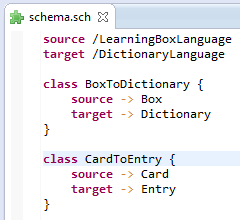
\includegraphics[width=0.4\textwidth]{eclipse_updatedSchema}
  \caption{Updating the schema}
  \label{eclipse:updatedSchema}
\end{center}
\end{figure}

\item[$\blacktriangleright$] Right-click on the \texttt{Rules} folder again, and create the \texttt{CardToEntryRule}.

\end{itemize}

One of the key differences between this rule and the last is that \texttt{CardToEntryRule} should only be invoked within a certain context i.e.,
this will only be used if a preexisting \texttt{partition} has \texttt{card} elements that need to be transformed into entries in an established
\texttt{dictionary}. In terms of MOSL, this means there will be both `black' and `green' elements.

\begin{itemize}

\item[$\blacktriangleright$] To begin, create three object variables in the \texttt{source} scope: \texttt{box}, \texttt{partition0}, and \texttt{card}. Which
ones are already known from the context? Which element still needs to be made? Your rule should come to resemble Fig.~\ref{eclipse:c2eRuleSource}.

\begin{figure}[htbp]
\begin{center}
  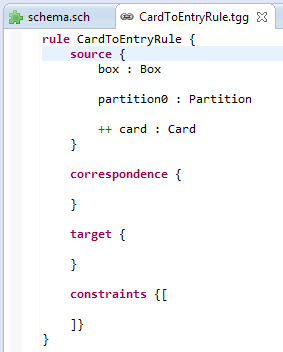
\includegraphics[width=0.45\textwidth]{eclipse_cardToEntry_sourceOVs}
  \caption{The source language with both `black' and `green' elements}
  \label{eclipse:c2eRuleSource}
\end{center}
\end{figure}

\item[$\blacktriangleright$] Similarly, in the \texttt{target} scope, you can declare \texttt{dictionary} from the context, but also need to create a new
entry object via \texttt{++ entry:Entry}. 

\vspace{0.5cm}

\item[$\blacktriangleright$] With all of our objects now created, we can complete the \texttt{correspondence}. Our contextual \texttt{box} and
\texttt{dictionary} objects can be connected via the same \texttt{boxToDictionary} link as declared in \texttt{BoxToDictionaryRule}, but a second link needs to
be created between \texttt{card} and \texttt{entry}. Use the correspondence type from the updated schema and write: \syntax{++ card <- cardToEntry : CardToEntry
-> entry}

% \begin{figure}[htbp]
% \begin{center}
%   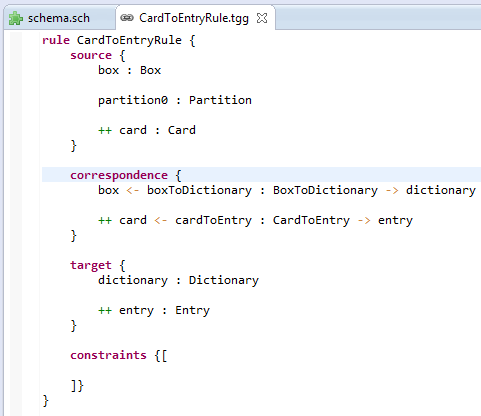
\includegraphics[width=0.8\textwidth]{eclipse_cardToEntry_correspondence}
%   \caption{correspondence}
%   \label{fig:c2etargetCorresp}
% \end{center}
% \end{figure}

\vspace{0.5cm}

\item[$\blacktriangleright$] Finally, let's make sure the transformation is able to access the \texttt{card} and \texttt{entry} attributes. Complete each
of your \texttt{box}, \texttt{partition0}, and \texttt{dictionary} object variable scopes with the relevant references until your rule matches
Fig.~\ref{eclipse:c2eAllReferences}.\footnote{Don't forget that eMoflon's type completion can help you establish references here; Press \texttt{ctrl + space
bar} after writing \texttt{->} for a list of available link variables from the relevant \texttt{eclass}.}

\newpage

\begin{figure}[htb]
\begin{center}
  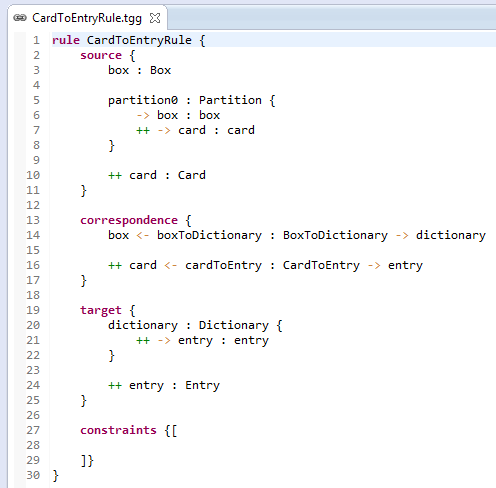
\includegraphics[width=0.8\textwidth]{eclipse_cardToEntry_objectVariables}
  \caption{all object variables}
  \label{eclipse:c2eAllReferences}
\end{center}
\end{figure}

\end{itemize}

Now let's establish the necessary \texttt{constraints} which will handle the relevant content attributes of \texttt{card} and \texttt{entry}. We'll need to
first decide on some common variables and syntax between \texttt{card.face}, \texttt{card.back}, and \texttt{entry.content} so that we can combine each side of
a \texttt{card} into one \texttt{content} value, or split each \texttt{entry} into a question and answer. 

\begin{itemize}

\item[$\blacktriangleright$] Define the syntax for \texttt{entry.content} as \texttt{<word>:<meaning>}, \texttt{card.back} as \texttt{Question:<word>}, and
\texttt{card.face} as \texttt{Answer:<meaning>}. Except perhaps on a piece of paper so you can keep track, there's no need to include this anywhere in the rule
-- the variable lifetimes will be exclusive to the constraint.

\vspace{0.5cm}

\item[$\blacktriangleright$] Now, using the preexisting String attribute constraint types, edit your \texttt{constraint} scope until it resembles
Fig.~\ref{eclipse:contentConstraints}.

\begin{figure}[htbp]
\begin{center}
  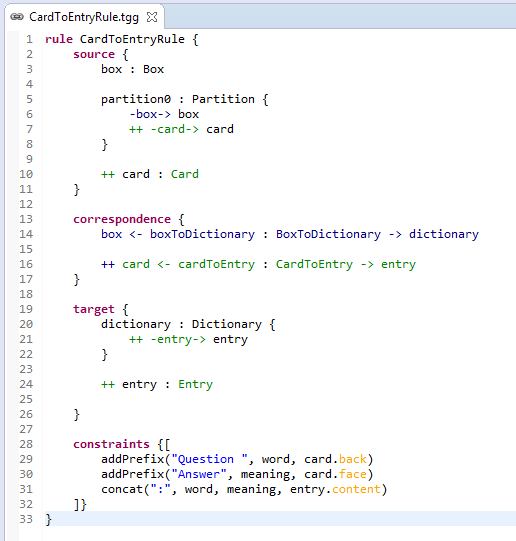
\includegraphics[width=0.8\textwidth]{eclipse_cardToEntry_firstConstraints}
  \caption{preexisting constraints}
  \label{eclipse:contentConstraints}
\end{center}
\end{figure}

\end{itemize}

\newpage

We're not quite done -- we need to add \emph{one} more constraint. Given that we have three partitions, and three difficulty levels for each \texttt{Entry}, why
don't we have the transformation assign a level based on whatever partition a \texttt{card} is found in? Hard cards, for example, are more likely to be found in the first
partition (due to being shifted backwards from wrong guesses), while easy cards will be near the end.  As you can imagine, there is no constraint type currently
existing in eMoflon to manage this. We must define our own!

\begin{itemize}

\item[$\blacktriangleright$] Add the following declaration to the \texttt{constraint} scope: \syntax{indexToLevel[BB,BF,FB](EInt, EString)} We will discuss what
each of the options mean in a moment.

\vspace{0.5cm}

\item[$\blacktriangleright$] You can now invoke your rule with \texttt{indexToLevel(partition0.index, entry.level)} immediately below the declaration. Your
completed \texttt{CardToEntryRule} should now resemble Fig.~\ref{eclipse:c2eDone}.

\begin{figure}[htbp]
\begin{center}
  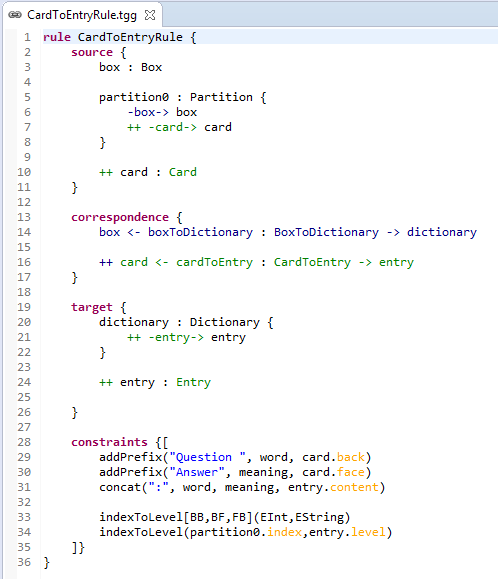
\includegraphics[width=0.9\textwidth]{eclipse_cardToEntry_complete}
  \caption{\texttt{CardToEntryRule complete!}}
  \label{eclipse:c2eDone}
\end{center}
\end{figure}

\vspace{0.5cm}

\item[$\blacktriangleright$] Awesome work! If you haven't already, save the file and confirm the MOSL parser hasn't raised any errors. Press \texttt{``Build
(Without Cleaning)''}, and admire your TGG transformation rules. 

\vspace{0.5cm}

\item[$\blacktriangleright$] To see how \texttt{BoxToDictionaryRule} is implemented in the visual syntax, check out Fig.~\ref{ea:boxtodictionaryrule_complete}
from Section 4.1. The \texttt{CardToEntryRule} is depicted in Fig.~\ref{ea:cardtoentry_complete} in Section 4.2.

\end{itemize}
